% fig_quad_rxplane.tex
% TR-34: R-X plane — Quad Zone 1/2 vs Mho Zone 1/2 for IBR lines
%
% Coordinate system:
%   X-axis: R_m [pu]  from -0.01 to 0.10
%   Y-axis: X_m [pu]  from -0.01 to 0.08
%
% Elements drawn:
%   Mho Zone 1: circle, centre (0, 0.020), radius 0.020  (grey dashed)
%   Mho Zone 2: circle, centre (0, 0.030), radius 0.030  (grey dotted)
%   Quad Zone 1: shaded rect [0..0.030] x [0..0.040]     (blue, light fill)
%   Quad Zone 2: shaded rect [0..0.050] x [0..0.060]     (teal, lighter)
%   Angle blinder 20°: line from origin                  (orange dashed)
%   Metallic fault locus: vertical line R=0, X in [0,0.05]
%   Resistive IBR locus (k=0.15, R_arc=0.008): R=0.0613, X in [0,0.05]
%   Load point (pf=0.95, Z_load~1.0 pu): far right — not plotted (OOB)

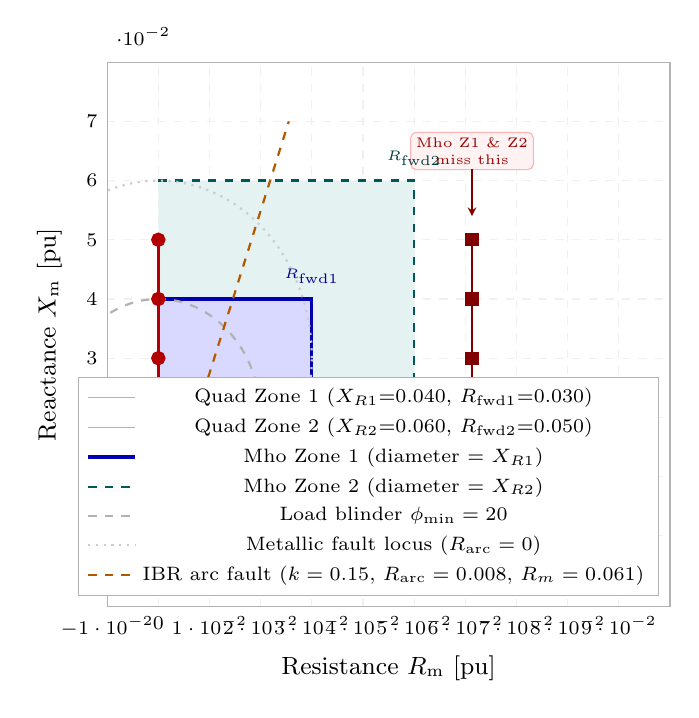
\begin{tikzpicture}[
  every node/.style = {font=\scriptsize},
]
\begin{axis}[
  name        = rxax,
  width       = 0.72\textwidth,
  height      = 8.5cm,
  xlabel      = {Resistance $R_\mathrm{m}$ [pu]},
  ylabel      = {Reactance $X_\mathrm{m}$ [pu]},
  xlabel style= {font=\small},
  ylabel style= {font=\small, yshift=2pt},
  xmin=-0.010, xmax=0.100,
  ymin=-0.012, ymax=0.080,
  xtick       = {-0.01,0,0.01,0.02,0.03,0.04,0.05,0.06,0.07,0.08,0.09},
  ytick       = {0,0.01,0.02,0.03,0.04,0.05,0.06,0.07},
  xticklabel style={font=\scriptsize},
  yticklabel style={font=\scriptsize},
  grid        = major,
  grid style  = {gray!12, dashed},
  tick style  = {draw=none},
  axis line style={gray!60},
  legend style={at={(0.98,0.02)}, anchor=south east, font=\tiny,
                draw=gray!60, fill=white},
]

%% ── Quad Zone 2 (background, teal) ──────────────────────────────────────────
\addplot[fill=teal!10, draw=none]
  coordinates {(0,0) (0.050,0) (0.050,0.060) (0,0.060)} \closedcycle;

%% ── Quad Zone 1 (foreground, blue) ──────────────────────────────────────────
\addplot[fill=blue!15, draw=none]
  coordinates {(0,0) (0.030,0) (0.030,0.040) (0,0.040)} \closedcycle;

%% ── Quad Zone 1 boundary ─────────────────────────────────────────────────────
\addplot[blue!70!black, very thick, mark=none]
  coordinates {(0,0.040) (0.030,0.040) (0.030,0) (0,0)};
\addlegendentry{Quad Zone~1 ($X_{R1}$=0.040, $R_\mathrm{fwd1}$=0.030)}

%% ── Quad Zone 2 boundary ─────────────────────────────────────────────────────
\addplot[teal!70!black, thick, mark=none, dashed]
  coordinates {(0,0.060) (0.050,0.060) (0.050,0) (0,0)};
\addlegendentry{Quad Zone~2 ($X_{R2}$=0.060, $R_\mathrm{fwd2}$=0.050)}

%% ── Mho Zone 1 circle (centre 0, 0.020), radius 0.020 ───────────────────────
%% Parametric: R=r*cos(t), X=r+r*sin(t), t in [-90°,90°] upper half
\addplot[gray!60, thick, dashed, mark=none,
         domain=0:360, samples=180]
  ({0.020*cos(x)}, {0.020 + 0.020*sin(x)});
\addlegendentry{Mho Zone~1 (diameter = $X_{R1}$)}

%% ── Mho Zone 2 circle (centre 0, 0.030), radius 0.030 ───────────────────────
\addplot[gray!40, thick, dotted, mark=none,
         domain=0:360, samples=180]
  ({0.030*cos(x)}, {0.030 + 0.030*sin(x)});
\addlegendentry{Mho Zone~2 (diameter = $X_{R2}$)}

%% ── Angle blinder 20° (line from origin) ─────────────────────────────────────
%% tan(20°) = 0.3640  → slope = X/R = 1/tan(20°) = 2.747
%% At R=0.090: X = 0.090*tan(70°) = 0.247... too far; clip to X=0.070 → R=0.070/tan(70°)=0.0255
\addplot[orange!70!black, thick, dashed, mark=none]
  coordinates {(0,0) (0.0255, 0.070)};
\addlegendentry{Load blinder $\phi_\mathrm{min}=20°$}

%% ── Metallic fault locus R=0 ─────────────────────────────────────────────────
\addplot[red!70!black, very thick, mark=*, mark size=2pt]
  coordinates {(0,0.010) (0,0.020) (0,0.030) (0,0.040) (0,0.050)};
\addlegendentry{Metallic fault locus ($R_\mathrm{arc}=0$)}

%% ── IBR resistive fault trajectory (k=0.15, R_arc=0.008, R_m=0.0613) ────────
\addplot[red!50!black, thick, mark=square*, mark size=2pt]
  coordinates {(0.0613,0.010) (0.0613,0.020) (0.0613,0.030)
               (0.0613,0.040) (0.0613,0.050)};
\addlegendentry{IBR arc fault ($k=0.15$, $R_\mathrm{arc}=0.008$, $R_m=0.061$)}

%% ── Annotation: Mho misses IBR arc fault ─────────────────────────────────────
\node[red!60!black, font=\tiny, align=center, draw=red!30, fill=red!5,
      rounded corners=2pt, inner sep=2pt]
  at (axis cs:0.0613, 0.065)
  {Mho Z1 \& Z2\\miss this};
\draw[->, >=stealth, red!50!black, thin]
  (axis cs:0.0613, 0.062) -- (axis cs:0.0613, 0.054);

%% ── R_fwd1 label ─────────────────────────────────────────────────────────────
\node[blue!60!black, font=\tiny, above=2pt]
  at (axis cs:0.030, 0.040) {$R_\mathrm{fwd1}$};

%% ── R_fwd2 label ─────────────────────────────────────────────────────────────
\node[teal!50!black, font=\tiny, above=2pt]
  at (axis cs:0.050, 0.060) {$R_\mathrm{fwd2}$};

%% ── Origin label ─────────────────────────────────────────────────────────────
\node[gray!60, font=\tiny, below left=1pt] at (axis cs:0,0) {O};

\end{axis}
\end{tikzpicture}
